\chapter{Năng lượng, động lượng và trường điện từ}

Bài giảng cuối cùng mở đầu bằng một sự sửa lại và kết thúc với đối tượng sẽ đứng ở vế phải của phương trình Einstein. Lộ trình này không phải là một đường vòng. Trước hết phải nói rõ một quy ước dấu cho điện trường; tiếp đó phải tách bạch ba nghĩa khác nhau của động lượng. Chỉ sau những bước chuẩn bị ấy mới có thể đọc lý thuyết trường như cơ học thông thường với một bậc tự do tại mỗi điểm trong không gian. Hamiltonian, mật độ năng lượng địa phương, động lượng Noether, năng lượng điện từ và vectơ Poynting rồi sẽ xuất hiện trong một lập luận liên tục duy nhất.

\section{Một quy ước phải được giữ nhất quán}

Các ghi chú sơ bộ vốn sẽ được đăng cho lớp, nhưng vấn đề này đủ quan trọng để giải quyết thành lời ngay tại lớp. Byron đã nhận ra một điểm không nhất quán không phải ở bên trong ký hiệu của khóa học, mà giữa ký hiệu đó với ký hiệu được dùng gần như ở khắp mọi nơi khác. Đây là một rủi ro nghề nghiệp của việc tự suy ra lại các phương trình từ đầu: một quy ước riêng tư nhất quán nội tại có thể trôi xa khỏi quy ước công khai.

Hãy viết \(\mathbf E_M\) cho quy ước Maxwell--Franklin chuẩn và \(\mathbf E_L\) cho quy ước đã dùng trong các bài giảng trước. Với thành phần hiệp biến \(A_0\) của khóa học, ta có
\begin{align}
\mathbf E_M
  &= -\dot{\mathbf A}+\boldsymbol{\nabla}A_0,
&
\mathbf E_L
  &= +\dot{\mathbf A}-\boldsymbol{\nabla}A_0
   =-\mathbf E_M .
\label{eq:two-electric-conventions}
\end{align}
Thay vào đó, nhiều sách đưa vào thế vô hướng \(\Phi=-A_0\); khi ấy công thức thứ nhất trở thành
\(\mathbf E_M=-\dot{\mathbf A}-\boldsymbol{\nabla}\Phi\).
Từ trường không thay đổi:
\begin{equation}
\mathbf B=\boldsymbol{\nabla}\times\mathbf A.
\label{eq:B-from-A-opening}
\end{equation}

Trong hệ đơn vị hữu tỉ hóa với \(c=1\), các phương trình Maxwell--Franklin chuẩn là
\begin{align}
\boldsymbol{\nabla}\times\mathbf E_M&=-\dot{\mathbf B},
&
\boldsymbol{\nabla}\cdot\mathbf B&=0,
\nonumber\\
\boldsymbol{\nabla}\times\mathbf B&=\dot{\mathbf E}_M+\mathbf J_F,
&
\boldsymbol{\nabla}\cdot\mathbf E_M&=\rho_F .
\label{eq:maxwell-franklin}
\end{align}
Lựa chọn lịch sử của Benjamin Franklin ấn định dấu của điện tích: electron là âm trong quy ước này. Quy ước của khóa học cũng đảo ngược các nhãn nguồn,
\begin{equation}
\mathbf J_L=-\mathbf J_F,
\qquad
\rho_L=-\rho_F.
\label{eq:source-convention-map}
\end{equation}
Vì vậy, thay \(\mathbf E_L=-\mathbf E_M\) vào ta được
\begin{align}
\boldsymbol{\nabla}\times\mathbf E_L&=+\dot{\mathbf B},
&
\boldsymbol{\nabla}\cdot\mathbf B&=0,
\nonumber\\
\boldsymbol{\nabla}\times\mathbf B&=-\dot{\mathbf E}_L-\mathbf J_L,
&
\boldsymbol{\nabla}\cdot\mathbf E_L&=\rho_L .
\label{eq:maxwell-course-convention}
\end{align}

\begin{figure}[H]
\centering

\includegraphics[width=\linewidth]{lecture_10_figure_01.png}
\caption{Đối chiếu đầy đủ trên bảng giữa quy ước Maxwell--Franklin và quy ước của khóa học.}
\par\smallskip
\textit{Khung hình bài giảng: 00:07:10.}
\end{figure}

Không có đại lượng đo được nào phụ thuộc vào việc chọn bảng đối chiếu nào. Điều quan trọng là tính nhất quán, đặc biệt khi một trường đã tính được được so sánh với một giá trị thực nghiệm đã công bố. Điều trớ trêu là những so sánh số trực tiếp như thế xuất hiện quá hiếm trong chính công việc của giảng viên, nên dấu ngược đã tồn tại mà không bị nhận ra cho đến khi lớp lưu ý đến nó. Đối với phép tính điện từ ở phần sau của chương này, ta sẽ dùng trường chuẩn
\(\mathbf E\equiv\mathbf E_M\).

\section{Ba đại lượng khác nhau cùng được gọi là động lượng}

Từ \emph{động lượng} giờ cần được tách bạch. Động lượng cơ học, động lượng chính tắc và động lượng Noether có thể trùng nhau trong những bài toán đơn giản, nhưng chúng không phải là ba cách mô tả của cùng một đại lượng. Trong một hệ tổng quát, chúng có thể có các giá trị số khác nhau.

\subsection{Động lượng cơ học}

Đối với một vật có tổng khối lượng \(M\), động lượng cơ học là
\begin{equation}
\mathbf P_{\mathrm{mech}}=M\dot{\mathbf X}_{\mathrm{cm}}.
\label{eq:mechanical-momentum}
\end{equation}
Đối với một hạt, \(\mathbf X_{\mathrm{cm}}\) đơn giản chính là vị trí của nó.
Đối với một vật hợp thành, việc nói rõ đó là khối tâm là điều thiết yếu.

\begin{figure}[H]
\centering
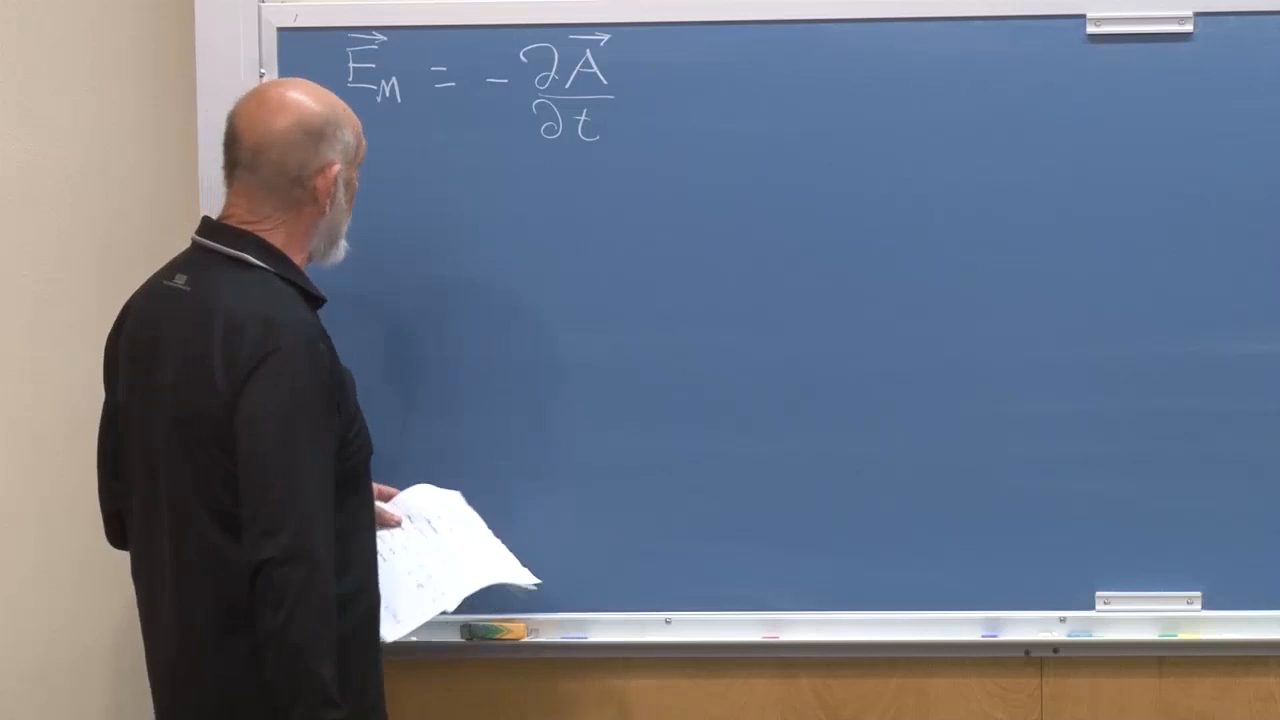
\includegraphics[width=\linewidth]{lecture_10_figure_02.png}
\caption{Động lượng cơ học được đưa vào như khối lượng nhân với vận tốc khối tâm.}
\par\smallskip
\textit{Khung hình bài giảng: 00:11:15.}
\end{figure}

\subsection{Động lượng chính tắc}

Giả sử cơ học được mô tả bởi
\(L(q_i,\dot q_i)\). Động lượng chính tắc liên hợp với \(q_i\) là
\begin{equation}
p_i=\frac{\partial L}{\partial\dot q_i}.
\label{eq:canonical-momentum}
\end{equation}
Với
\begin{equation}
L=\frac12 m\dot{\mathbf x}^{\,2}-V(\mathbf x),
\label{eq:simple-particle-lagrangian}
\end{equation}
thì ta được \(\mathbf p=m\dot{\mathbf x}\), nên động lượng chính tắc và động lượng cơ học tình cờ trùng nhau.

\begin{figure}[H]
\centering
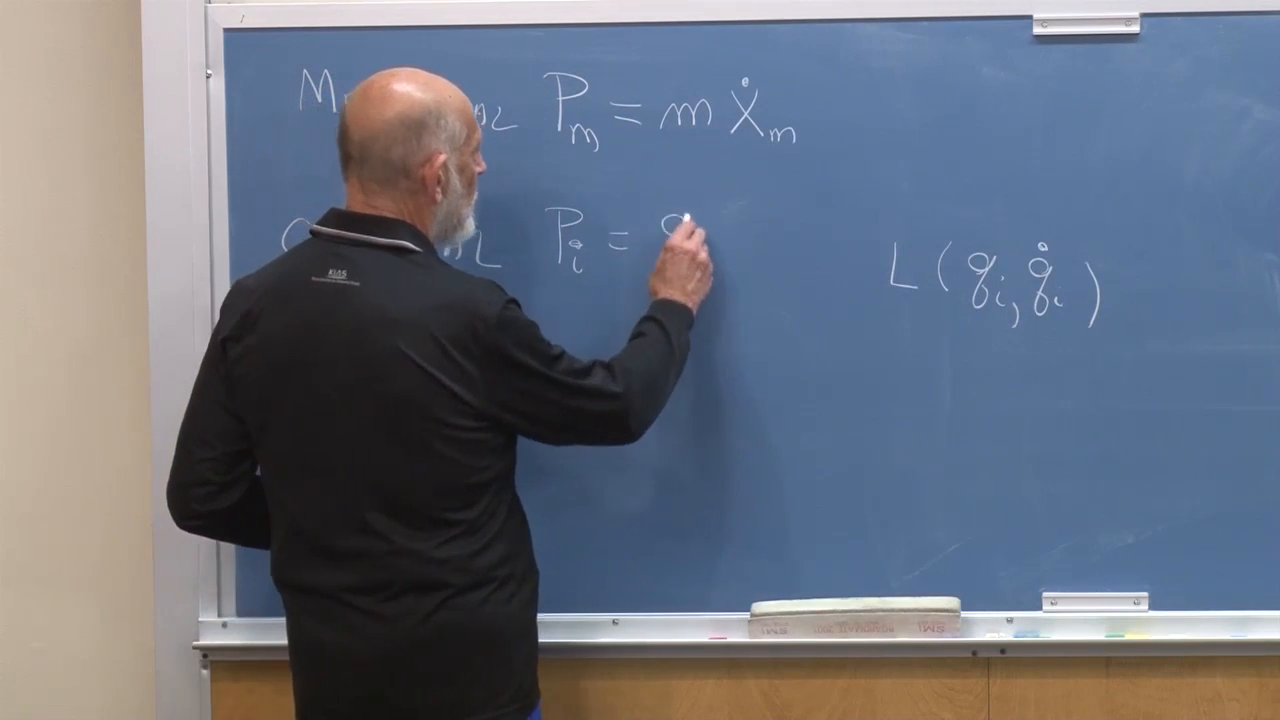
\includegraphics[width=\linewidth]{lecture_10_figure_03.png}
\caption{Động lượng cơ học và động lượng chính tắc được trình bày bên cạnh Lagrangian hạt đơn giản.}
\par\smallskip
\textit{Khung hình bài giảng: 00:13:40.}
\end{figure}

Một hạt mang điện trong từ trường là phản ví dụ hữu ích. Với quy ước dấu được viết trên bảng,
\begin{equation}
L=\frac12m\dot{\mathbf x}^{\,2}-V(\mathbf x)
  -e\,\dot{\mathbf x}\cdot\mathbf A(\mathbf x),
\label{eq:magnetic-particle-lagrangian}
\end{equation}
và do đó
\begin{equation}
p_i=m\dot x_i-eA_i.
\label{eq:magnetic-canonical-shift}
\end{equation}
Việc thay đổi quy ước cho điện tích hoặc cho hạng tương tác sẽ làm đổi dấu được viết ra, nhưng không làm thay đổi bài học rút ra: động lượng chính tắc chứa một phần đóng góp của thế vectơ và không chỉ đơn thuần là \(m\dot x_i\).
Các phương trình Hamilton dùng biến chính tắc. Về sau ta có thể chuyển hạng phụ thuộc trường sang vế kia của một phương trình và khôi phục một gia tốc có dạng Newton, nhưng sự sắp xếp lại đó không làm thay đổi định nghĩa.

\begin{figure}[H]
\centering
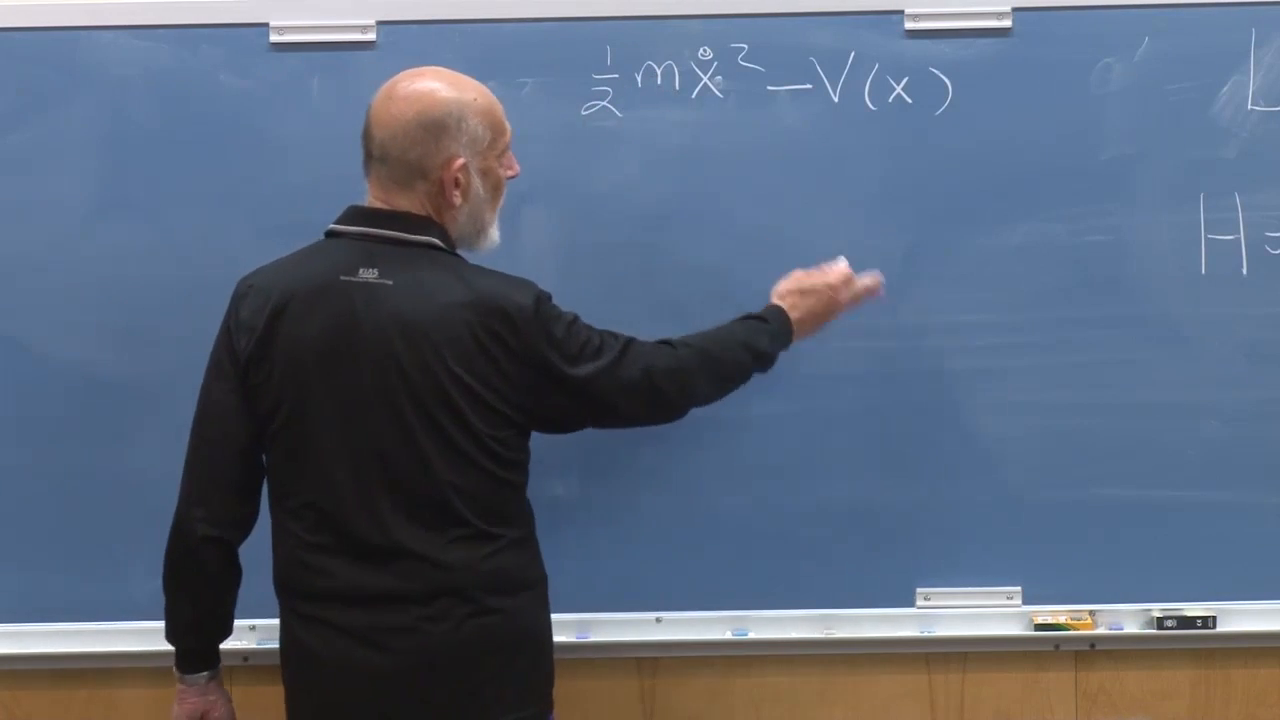
\includegraphics[width=\linewidth]{lecture_10_figure_04.png}
\caption{Hạng thế vectơ làm dịch động lượng chính tắc khỏi động lượng cơ học.}
\par\smallskip
\textit{Khung hình bài giảng: 00:15:50.}
\end{figure}

\subsection{Động lượng Noether}

Động lượng thứ ba là đại lượng bảo toàn gắn với tính bất biến đối với tịnh tiến không gian. Đối với một đối xứng vô cùng bé
\begin{equation}
q_i\longrightarrow q_i+\delta q_i
\end{equation}
làm Lagrangian bất biến, định lý Noether cho, tính đến cách chuẩn hóa của tham số vô cùng bé,
\begin{equation}
Q=\sum_i p_i\,\delta q_i.
\label{eq:noether-charge-mechanics}
\end{equation}
Các \(p_i\) xuất hiện ở đây là các động lượng chính tắc. Nếu đối xứng là một phép tịnh tiến đều và động lượng chính tắc tình cờ bằng động lượng cơ học, thì \(Q\) thu về động lượng toàn phần quen thuộc. Trong một hệ kém đơn giản hơn, sự trùng nhau đó phải được chứng minh, không được giả định.

\begin{figure}[H]
\centering
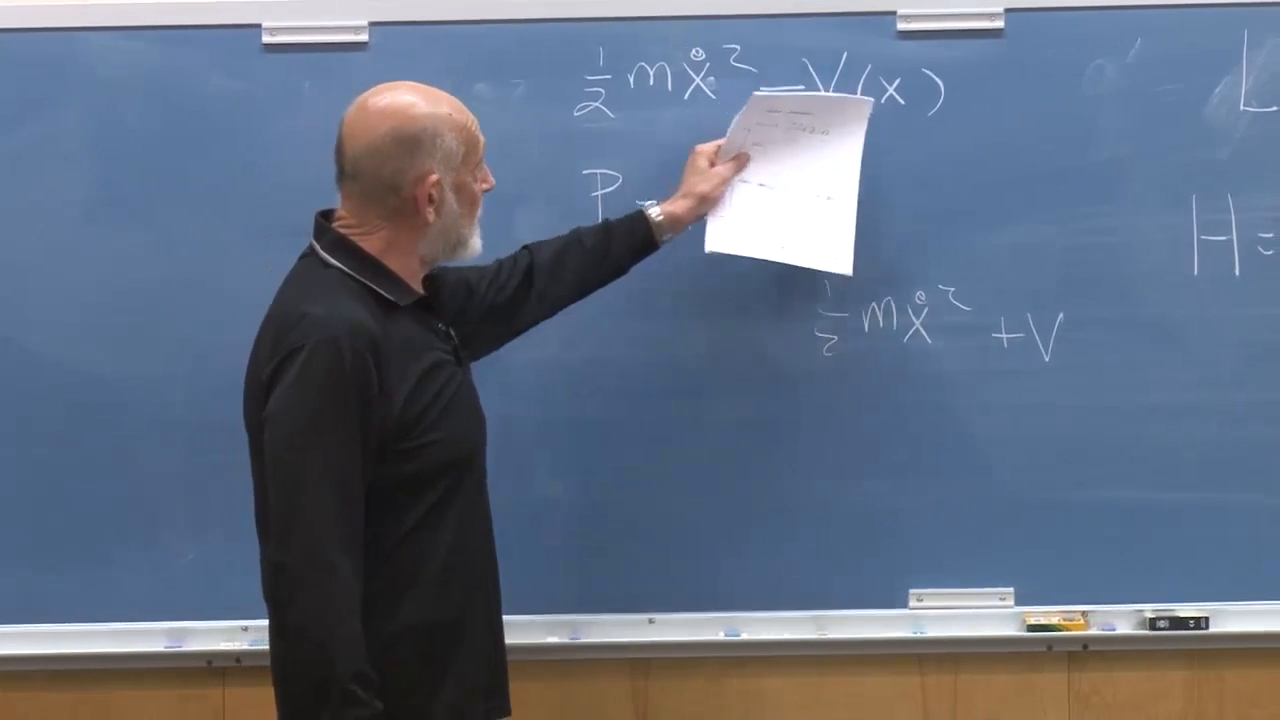
\includegraphics[width=\linewidth]{lecture_10_figure_05.png}
\caption{Điện tích Noether được ghép từ các động lượng chính tắc và các biến thiên vô cùng bé của các tọa độ.}
\par\smallskip
\textit{Khung hình bài giảng: 00:19:00.}
\end{figure}

\section{Năng lượng là Hamiltonian}

Tịnh tiến không gian dẫn tới động lượng; tịnh tiến thời gian dẫn tới năng lượng. Nếu Lagrangian không phụ thuộc tường minh vào thời gian, thì Hamiltonian
\begin{equation}
H=\sum_i p_i\dot q_i-L
\label{eq:hamiltonian-definition}
\end{equation}
được bảo toàn. Đây là biến đổi Legendre của Lagrangian, không phải một quy tắc đổi dấu chỉ bằng quan sát.

\begin{figure}[H]
\centering
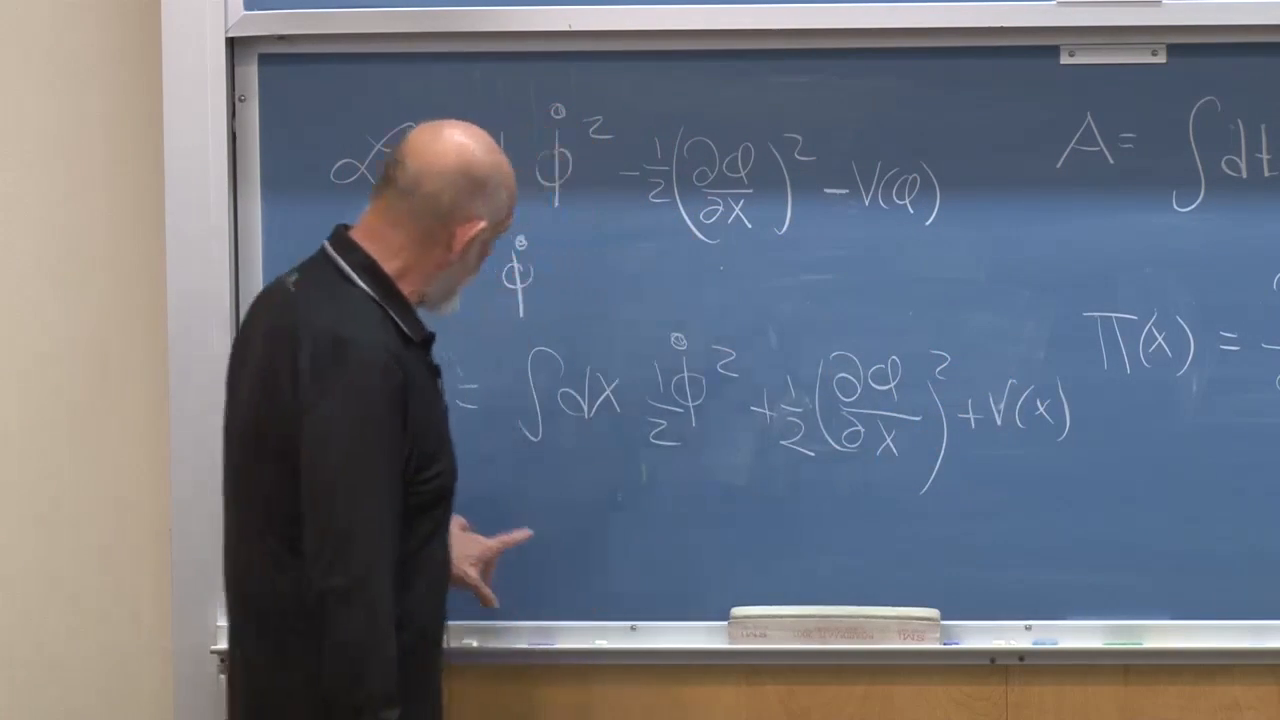
\includegraphics[width=\linewidth]{lecture_10_figure_06.png}
\caption{Hamiltonian được viết như biến đổi Legendre của một Lagrangian tổng quát.}
\par\smallskip
\textit{Khung hình bài giảng: 00:22:55.}
\end{figure}

Đối với ví dụ một hạt,
\begin{align}
p&=m\dot x,
\nonumber\\
H&=p\dot x-L\\
&=m\dot x^2
  -\left(\frac12m\dot x^2-V(x)\right)\\
&=\frac12m\dot x^2+V(x).
\label{eq:particle-hamiltonian}
\end{align}
Vì vậy, Lagrangian là động năng trừ thế năng, còn Hamiltonian là động năng cộng thế năng.

\begin{figure}[H]
\centering
\includegraphics[width=\linewidth]{lecture_10_figure_07.png}
\caption{Phép tính cho hạt cho thấy \(H=T+V\) suy ra từ \(H=p\dot x-L\) như thế nào.}
\par\smallskip
\textit{Khung hình bài giảng: 00:24:20.}
\end{figure}

Khi mọi phụ thuộc vào vận tốc đều là một hạng động năng bậc hai dương thông thường và phần còn lại không chứa vận tốc, ta có thể suy ra Hamiltonian bằng cách đổi dấu phần không phụ thuộc vận tốc. Lối tắt đó sẽ được dùng lặp đi lặp lại. Nó chỉ an toàn vì biến đổi Legendre có dạng đơn giản này trong các ví dụ đang xét.

\section{Một trường là một hệ cơ học với một số liên tục các tọa độ}

Để làm lộ ra cấu trúc cơ học của lý thuyết trường, hãy chọn một hệ quy chiếu quán tính và tạm thời đừng khăng khăng rằng mọi dòng đều biểu lộ hiệp biến Lorentz một cách tường minh. Cơ học cổ điển có một trục thời gian và các tọa độ \(q_i(t)\). Một trường vô hướng có một trục thời gian và các tọa độ \(\phi(\mathbf x,t)\). Nhãn rời rạc \(i\) đơn giản đã trở thành nhãn liên tục \(\mathbf x\):
\begin{equation}
q_i(t)\quad\longrightarrow\quad\phi(\mathbf x,t).
\label{eq:discrete-to-field}
\end{equation}
Giá trị của trường tại mỗi điểm không gian là một bậc tự do. Ở đây \(\mathbf x\) gắn nhãn bậc tự do đang được nói tới; bản thân nó không phải là tọa độ suy rộng.

\begin{figure}[H]
\centering
\includegraphics[width=\linewidth]{lecture_10_figure_08.png}
\caption{Một mạng điểm không gian được dùng để biểu diễn giá trị trường tại mỗi điểm như một bậc tự do cơ học riêng biệt.}
\par\smallskip
\textit{Khung hình bài giảng: 00:30:15.}
\end{figure}

\begin{classroomqa}
\audiencequestion{Tại sao không viết trường là \(\phi(\mathbf x,t)\) ngay từ đầu?}
\lecturerresponse{Đó là ký hiệu đầy đủ. Ký hiệu tạm thời \(\phi(\mathbf x)\) lược bỏ đối số thời gian chung, cũng như người ta thường viết \(q_i\) nhưng vẫn nhớ rằng mọi \(q_i\) đều phụ thuộc vào thời gian. Nhãn \(i\), hay bây giờ là \(\mathbf x\), cho ta biết bậc tự do nào đang được bàn tới. \lecturetimestamp{00:32:43}}
\end{classroomqa}

\begin{classroomqa}
\audiencequestion{Các giá trị của trường tại những điểm lân cận có thật sự là các tọa độ độc lập không? Điều gì áp đặt tính liên tục?}
\lecturerresponse{Chúng là các tọa độ chính tắc độc lập. Tính trơn không được áp đặt bằng cách đồng nhất các giá trị lân cận; nó được chọn ra bởi động lực học. Hamiltonian chứa một hạng năng lượng gradient dương, nên một độ nhảy cố định trên một khoảng cách ngày càng nhỏ sẽ tốn năng lượng ngày càng lớn. Vì thế, các cấu hình năng lượng hữu hạn là trơn trong giới hạn liên tục. \lecturetimestamp{00:33:09}}
\end{classroomqa}

Một đạo hàm không gian làm cho sự ghép giữa các bậc tự do lân cận trở nên tường minh. Trên một mạng có khoảng cách \(\epsilon\),
\begin{equation}
\partial_x\phi(x,t)
  =\lim_{\epsilon\to0}
   \frac{\phi(x+\epsilon,t)-\phi(x,t)}{\epsilon}.
\label{eq:field-finite-difference}
\end{equation}
Nó phụ thuộc vào hai tọa độ gần nhau, nhưng không chứa vận tốc suy rộng nào. Trong phép tương tự cơ học, nó thuộc về phần phụ thuộc theo tọa độ của Lagrangian, chứ không thuộc về phần phụ thuộc theo \(\dot q_i\).

\begin{figure}[H]
\centering
\includegraphics[width=\linewidth]{lecture_10_figure_09.png}
\caption{Đạo hàm không gian được dựng lại thành hiệu trường giữa các điểm lân cận trên mạng.}
\par\smallskip
\textit{Khung hình bài giảng: 00:31:40.}
\end{figure}

Tác dụng giờ có thể được viết dưới dạng cơ học tường minh:
\begin{align}
S&=\int dt\,L,
\nonumber\\
L&=\int d^3x\,
\mathcal L\!\left(
\phi,\dot\phi,\boldsymbol{\nabla}\phi
\right),
\nonumber\\
S&=\int dt\,d^3x\,
\mathcal L\!\left(
\phi,\dot\phi,\boldsymbol{\nabla}\phi
\right).
\label{eq:field-action-split}
\end{align}
Ký tự script \(\mathcal L\) là mật độ Lagrangian; lấy tích phân của nó theo không gian cho Lagrangian thông thường, rồi Lagrangian ấy được tích phân theo thời gian. Một lý thuyết địa phương chỉ ghép mỗi điểm thông qua các trường và các đạo hàm của chúng tại chính điểm đó. Việc tách thời gian ra khỏi không gian tạm thời che đi hiệp biến Lorentz, nhưng làm cho cơ học trở nên minh bạch.

\begin{figure}[H]
\centering
\includegraphics[width=\linewidth]{lecture_10_figure_10.png}
\caption{Tác dụng của trường được tách thành một tích phân theo thời gian và một tích phân theo không gian của mật độ Lagrangian.}
\par\smallskip
\textit{Khung hình bài giảng: 00:36:40.}
\end{figure}

\section{Động lượng trường chính tắc và mật độ Hamiltonian}

Vận tốc của một tọa độ trường là \(\dot\phi(\mathbf x,t)\): đó là tốc độ mà trường biến thiên theo thời gian tại một điểm cố định. Nó không phải là chuyển động từ điểm không gian này sang điểm khác. Do đó, động lượng chính tắc liên hợp với trường bản thân cũng là một trường,
\begin{equation}
\Pi(\mathbf x,t)
 =\frac{\partial\mathcal L}{\partial\dot\phi(\mathbf x,t)}.
\label{eq:field-canonical-momentum}
\end{equation}
Đối với nhiều trường \(\phi_a\), có một trường động lượng \(\Pi_a\) cho mỗi trường.

Tổng rời rạc trong biến đổi Legendre trở thành một tích phân theo không gian:
\begin{align}
H
 &=\int d^3x\,
   \left[\Pi\dot\phi-\mathcal L\right]
  =\int d^3x\,\mathcal H,
\nonumber\\
\mathcal H
 &=\Pi\dot\phi-\mathcal L .
\label{eq:field-hamiltonian-density}
\end{align}
Đại lượng nằm trong dấu tích phân là mật độ năng lượng.

\begin{figure}[H]
\centering
\includegraphics[width=\linewidth]{lecture_10_figure_11.png}
\caption{Biến đổi Legendre của trường và cách hiểu nó như một tích phân của mật độ năng lượng địa phương.}
\par\smallskip
\textit{Khung hình bài giảng: 00:42:40.}
\end{figure}

\begin{classroomqa}
\audiencequestion{Tại sao đạo hàm của toàn bộ Lagrangian theo \(\dot\phi\) tại một điểm lại có thể được thay bằng đạo hàm của mật độ địa phương tại đó?}
\lecturerresponse{Hãy nghĩ tích phân theo không gian như một tổng liên tục. Dưới giả thiết địa phương được dùng ở đây, vận tốc \(\dot\phi(\mathbf x)\) chỉ xuất hiện trong hạng thuộc về chính điểm đó. Việc lấy đạo hàm theo vận tốc cụ thể ấy loại bỏ tất cả các hạng khác. Các đạo hàm không gian có thể ghép các giá trị trường lân cận, nhưng trong lý thuyết này chúng không đưa vào các đạo hàm thời gian lân cận. \lecturetimestamp{00:51:56}}
\end{classroomqa}

\subsection{Trường vô hướng}

Trong một chiều không gian, lấy
\begin{equation}
\mathcal L
 =\frac12\dot\phi^2
  -\frac12(\partial_x\phi)^2
  -V(\phi).
\label{eq:scalar-field-lagrangian}
\end{equation}
Đây là cách viết không hiệp biến của vô hướng Lorentz đã dùng trước đó: dấu trừ tương đối giữa đạo hàm theo thời gian và đạo hàm theo không gian đến từ metric Minkowski. Động lượng chính tắc là
\begin{equation}
\Pi=\dot\phi,
\label{eq:scalar-pi}
\end{equation}
và Hamiltonian trở thành
\begin{equation}
H=\int dx\,
\left[
\frac12\dot\phi^2
+\frac12(\partial_x\phi)^2
+V(\phi)
\right].
\label{eq:scalar-field-hamiltonian}
\end{equation}
Trong lúc tính toán, thế có lúc tạm được gọi là \(V(x)\); cả lớp đã sửa lại thành \(V(\phi)\). Nó có thể phụ thuộc vào vị trí một cách gián tiếp thông qua trường, nhưng trong lý thuyết bất biến đối với tịnh tiến thì nó không có sự phụ thuộc ngoài được ấn định sẵn theo \(x\).

\begin{figure}[H]
\centering
\includegraphics[width=\linewidth]{lecture_10_figure_12.png}
\caption{Mật độ Lagrangian vô hướng, động lượng liên hợp và Hamiltonian dương được tập hợp trên cùng một bảng.}
\par\smallskip
\textit{Khung hình bài giảng: 00:47:05.}
\end{figure}

Toàn bộ phần không chứa đạo hàm theo thời gian đóng vai trò của năng lượng thế. Phần đó bao gồm cả \(V(\phi)\) lẫn năng lượng gradient \(\frac12(\partial_x\phi)^2\). Lagrangian có thể mang dấu nào cũng được; còn một năng lượng ổn định thì phải được chặn dưới.

\begin{classroomqa}
\audiencequestion{Thế \(V(\phi)\) có thể âm không?}
\lecturerresponse{Có. Nếu nó có một cận dưới hữu hạn, ta có thể cộng thêm một hằng số để giá trị nhỏ nhất của nó bằng không mà không làm thay đổi phương trình trường cổ điển. Một thế không bị chặn dưới mô tả một bất ổn định: trường có thể hạ năng lượng của nó xuống vô hạn. Chân không ổn định là một trường hằng nằm tại một cực tiểu của thế đã được tịnh tiến.
\lecturetimestamp{00:49:03}}
\end{classroomqa}

Câu hỏi trước đó về tính liên tục nay được trả lời một cách định lượng. Một bước nhảy \(\Delta\phi\) qua một khoảng cách mạng \(\epsilon\) đóng góp
\begin{equation}
\frac12(\partial_x\phi)^2
\sim\frac12\left(\frac{\Delta\phi}{\epsilon}\right)^2.
\label{eq:gradient-cost}
\end{equation}
Khi \(\epsilon\to0\), một bước nhảy cố định cho một mật độ năng lượng lớn tùy ý. Vì vậy, năng lượng hữu hạn sẽ triệt bớt các cấu hình gấp khúc.

\begin{figure}[H]
\centering
\includegraphics[width=\linewidth]{lecture_10_figure_13.png}
\caption{Biểu thức năng lượng của trường vô hướng được giữ lại, trong khi hình phác trên bảng đối chiếu một trường trơn với một biến thiên đột ngột.}
\par\smallskip
\textit{Khung hình bài giảng: 00:54:20.}
\end{figure}

\section{Năng lượng cục bộ và ý nghĩa của \texorpdfstring{\(T^{00}\)}{T00}}

Mật độ năng lượng có một tên gọi gọn:
\begin{equation}
T^{00}=\mathcal H=\Pi\dot\phi-\mathcal L.
\label{eq:T00-definition}
\end{equation}
Hai chỉ số 0 mã hóa hai mệnh đề riêng biệt. Năng lượng là thành phần thời gian \(P^0\) của bốn-vectơ năng lượng--động lượng, còn một mật độ là thành phần thời gian của một dòng bảo toàn. Do đó \(T^{00}\) là mật độ của thành phần thời gian của bốn-động lượng.

\begin{figure}[H]
\centering
\includegraphics[width=\linewidth]{lecture_10_figure_14.png}
\caption{Năng lượng của trường được viết dưới dạng cục bộ và được đồng nhất với
\(T^{00}\).}
\par\smallskip
\textit{Khung hình bài giảng: 01:00:00.}
\end{figure}

Sự bảo toàn trong một lý thuyết địa phương tương đối tính không chỉ đơn thuần là phát biểu rằng một đại lượng toàn cục nào đó vẫn không đổi. Năng lượng không thể biến mất trong phòng thí nghiệm rồi xuất hiện lại ở Alpha Centauri. Một biến thiên bên trong một miền phải được giải thích bằng một thông lượng qua biên của miền ấy. Ở dạng địa phương,
\begin{equation}
\partial_\mu T^{\mu\nu}=0,
\label{eq:stress-energy-continuity}
\end{equation}
nên chỉ số thứ nhất gắn nhãn mật độ hoặc hướng thông lượng, còn chỉ số thứ hai gắn nhãn thành phần \(P^\nu\) nào đang được vận chuyển.

\begin{classroomqa}
\audiencequestion{Việc gọi \(T^{00}\) là một mật độ có nghĩa là tổng năng lượng thu được bằng cách lấy tích phân của nó sao?}
\lecturerresponse{Chính xác:
\(E=P^0=\int d^3x\,T^{00}\). Mật độ địa phương là biểu thức dưới dấu tích phân trong phép biến đổi Legendre của trường. Sự biến thiên của nó tại một chỗ được cân bằng bởi một dòng năng lượng qua các vị trí lân cận. \lecturetimestamp{00:59:06}}
\end{classroomqa}

\section{Mật độ động lượng từ các phép tịnh tiến không gian}

Quay lại công thức của Noether, giờ thay tổng rời rạc bằng một tích phân không gian. Dưới một phép tịnh tiến nhỏ theo hướng \(m\), trường biến đổi theo
\begin{equation}
\delta\phi
  =\phi(\mathbf x)-\phi(\mathbf x-\boldsymbol{\epsilon})
  =\epsilon^m\partial_m\phi+O(\epsilon^2),
\label{eq:translated-field-change}
\end{equation}
theo quy ước thụ động được dùng trên bảng. Việc đảo giữa tịnh tiến chủ động và thụ động sẽ đảo dấu tổng thể; bộ sinh vật lý được cố định một khi đã chọn quy ước đó. Tách \(\epsilon^m\) ra, động lượng Noether có cấu trúc
\begin{equation}
P_m\ \propto\ \int d^3x\,\Pi\,\partial_m\phi.
\label{eq:scalar-noether-momentum}
\end{equation}

\begin{figure}[H]
\centering
\includegraphics[width=\linewidth]{lecture_10_figure_15.png}
\caption{Một biên dạng trường đã tịnh tiến và đạo hàm đo sự biến đổi vô cùng bé của nó.}
\par\smallskip
\textit{Khung hình bài giảng: 01:04:20.}
\end{figure}

\begin{classroomqa}
\audiencequestion{Vì sao phép tịnh tiến vô cùng bé
\(\epsilon\) không được giữ lại trong công thức động lượng?}
\lecturerresponse{Điện tích Noether ban đầu thu được tỉ lệ với
\(\epsilon\). Động lượng được định nghĩa là hệ số của tham số tịnh tiến tùy ý đó, nên \(\epsilon\) được chia ra. Nhân một đại lượng bảo toàn với một hằng số cố định sẽ không ảnh hưởng đến tính bảo toàn, nhưng việc tách hệ số ra cho chuẩn hóa tiêu chuẩn.
\lecturetimestamp{01:04:45}}
\end{classroomqa}

\begin{classroomqa}
\audiencequestion{Khoảng tịnh tiến có trở thành \(dx\) trong tích phân liên tục không?}
\lecturerresponse{Chúng xuất hiện từ những giới hạn khác nhau. Phần tử đo \(dx\) đến từ việc thay tổng trên các bậc tự do được gắn nhãn theo không gian bằng một tích phân. Tham số tịnh tiến \(\epsilon\) mô tả phép đối xứng và được tách ra khỏi điện tích Noether của nó. Cả hai đều là vô cùng bé trong lập luận trung gian, nhưng chúng giữ những vai trò khác nhau.
\lecturetimestamp{01:05:16}}
\end{classroomqa}

Theo ký hiệu của bài giảng, mật độ của thành phần \(m\) của động lượng là
\begin{equation}
T^{0m}=\Pi\,\partial_m\phi,
\label{eq:scalar-momentum-density}
\end{equation}
theo quy ước dấu của phép tịnh tiến đã được ngầm hiểu. Đối với lý thuyết vô hướng, \(\Pi=\dot\phi\), nên nó tỉ lệ với
\(\dot\phi\,\partial_m\phi\).

\begin{figure}[H]
\centering
\includegraphics[width=\linewidth]{lecture_10_figure_16.png}
\caption{Mật độ động lượng Noether
\(T^{0m}=\Pi\,\partial_m\phi\) trên bảng.}
\par\smallskip
\textit{Khung hình bài giảng: 01:07:10.}
\end{figure}

Đây là động lượng theo nghĩa đen do một sóng mang theo. Tính bất biến tịnh tiến chỉ áp dụng khi mọi thứ đều được tịnh tiến: các trường, các hạt, các nguồn và thiết bị. Một xung ánh sáng bị hấp thụ bởi một tấm bảng được treo tự do sẽ làm tấm bảng giật lùi. Ánh sáng thông thường làm hiệu ứng này rất nhỏ; một laser đủ mạnh có thể truyền đủ động lượng để nén một mục tiêu nhỏ. Đại lượng tổng được bảo toàn thuộc về các hạt và các trường cùng nhau.

\subsection{Điều gì thay thế phương trình Newton?}

Phương trình trường Euler--Lagrange suy ra từ phương trình~\eqref{eq:scalar-field-lagrangian} là
\begin{equation}
\ddot\phi-\nabla^2\phi=-\frac{dV}{d\phi}.
\label{eq:scalar-equation-of-motion}
\end{equation}
Nó là tương tự trong lý thuyết trường của định luật Newton.

\begin{figure}[H]
\centering
\includegraphics[width=\linewidth]{lecture_10_figure_17.png}
\caption{Phương trình trường vô hướng được trình bày bên cạnh Hamiltonian và mật độ động lượng của nó.}
\par\smallskip
\textit{Khung hình bài giảng: 01:12:55.}
\end{figure}

\begin{classroomqa}
\audiencequestion{Đối với một trường, cái gì tương ứng với định luật Newton?}
\lecturerresponse{Chính là phương trình trường Euler--Lagrange. Ở đây nó là một phương trình sóng với hạng lực \(-V'(\phi)\). Vai trò của
\(m\ddot x=-V'(x)\) được đảm nhiệm bởi
\(\ddot\phi-\nabla^2\phi=-V'(\phi)\).
\lecturetimestamp{01:11:48}}
\end{classroomqa}

\begin{classroomqa}
\audiencequestion{Làm sao ta biết một Lagrangian trường được đề xuất là đúng? Có nhất thiết ta phải biết trước phương trình trường không?}
\lecturerresponse{Có thể đi theo cả hai hướng. Về mặt lịch sử, ta có thể suy ra các phương trình từ thực nghiệm rồi tìm một tác dụng, như đã xảy ra với Newton và Maxwell. Trong lý thuyết hiện đại, người ta thường bắt đầu từ nội dung trường, tính địa phương, đối xứng và một tập nhỏ các hạng được phép, suy ra các phương trình rồi kiểm tra các dự đoán của chúng. Trường vô hướng được viết ra có thể mô tả một trường cơ bản, nhưng cũng có thể mô tả độ dời ngang của một sợi dây mà tác dụng liên tục của nó được suy ra từ các hạt cấu thành. \lecturetimestamp{01:12:55}}
\end{classroomqa}

\section{Trường điện từ trong chuẩn thời gian}

Các thành phần đã tìm được,
\(T^{00}\) và \(T^{0m}\), thuộc về tenxơ năng lượng--động lượng. Các thành phần còn lại của nó mô tả thông lượng năng lượng và động lượng. Về sau tenxơ này sẽ làm nguồn cho hấp dẫn, nhưng điện từ học cung cấp ví dụ trực tiếp trước mắt.

Biến tọa độ điện từ cơ bản là bốn-thế \(A_\mu\).
Tự do chuẩn cho phép
\begin{equation}
A_\mu\longrightarrow A'_\mu=A_\mu+\partial_\mu S
\label{eq:gauge-transformation-lecture10}
\end{equation}
mà không làm thay đổi \(F_{\mu\nu}\). Chọn \(S\) sao cho thỏa mãn
\begin{equation}
\partial_tS=-A_0.
\label{eq:temporal-gauge-choice}
\end{equation}
Ví dụ, tại mỗi điểm không gian cố định, ta có thể lấy tích phân \(A_0\) theo thời gian. Khi đó thành phần thời gian sau biến đổi triệt tiêu:
\begin{equation}
A'_0=A_0+\partial_tS=0.
\label{eq:temporal-gauge}
\end{equation}
Đây là chuẩn thời gian. Nó loại \(A_0\) khỏi danh sách các tọa độ động lực, mặc dù định luật Gauss vẫn còn như một ràng buộc và vẫn còn một tự do chuẩn dư độc lập với thời gian.

\begin{figure}[H]
\centering
\includegraphics[width=\linewidth]{lecture_10_figure_18.png}
\caption{Tự do chuẩn được dùng để chọn \(A_0=0\) bằng cách giải
\(\partial_tS=-A_0\).}
\par\smallskip
\textit{Khung hình bài giảng: 01:20:15.}
\end{figure}

Từ điểm này trở đi, hãy để \(\mathbf E\) ký hiệu điện trường Maxwell theo quy ước chuẩn. Trước khi cố định chuẩn,
\begin{equation}
E_m=-\partial_tA_m+\partial_mA_0,
\qquad
\mathbf B=\boldsymbol{\nabla}\times\mathbf A.
\label{eq:E-B-general-potential}
\end{equation}
Trong chuẩn thời gian, các biểu thức này rút gọn thành
\begin{equation}
\mathbf E=-\dot{\mathbf A},
\qquad
\mathbf B=\boldsymbol{\nabla}\times\mathbf A.
\label{eq:E-B-temporal-gauge}
\end{equation}
Các đạo hàm theo thời gian của \(\mathbf A\) cho ra điện trường; các đạo hàm theo không gian cho ra từ trường.

\begin{figure}[H]
\centering
\includegraphics[width=\linewidth]{lecture_10_figure_19.png}
\caption{Điện trường và từ trường trong chuẩn thời gian:
\(\mathbf E=-\dot{\mathbf A}\) và
\(\mathbf B=\nabla\times\mathbf A\).}
\par\smallskip
\textit{Khung hình bài giảng: 01:23:50.}
\end{figure}

\section{Động lượng chính tắc và năng lượng điện từ}

Mật độ Lagrangian Maxwell tự do là
\begin{equation}
\mathcal L_{\mathrm{EM}}
 =-\frac14F_{\mu\nu}F^{\mu\nu}
 =\frac12\left(\mathbf E^2-\mathbf B^2\right).
\label{eq:maxwell-lagrangian-energy-lecture}
\end{equation}
Trong chuẩn thời gian,
\begin{equation}
\mathcal L_{\mathrm{EM}}
 =\frac12\dot{\mathbf A}^{\,2}
  -\frac12(\boldsymbol{\nabla}\times\mathbf A)^2.
\label{eq:maxwell-lagrangian-temporal}
\end{equation}
Nó có đúng mẫu hình của trường vô hướng: bình phương các đạo hàm theo thời gian trừ đi bình phương các đạo hàm theo không gian.

\begin{figure}[H]
\centering
\includegraphics[width=\linewidth]{lecture_10_figure_20.png}
\caption{Lagrangian Maxwell được viết lại như một Lagrangian trường cơ học cho các thành phần không gian của \(\mathbf A\).}
\par\smallskip
\textit{Khung hình bài giảng: 01:28:10.}
\end{figure}

Mỗi thành phần \(A_m\) có một động lượng chính tắc,
\begin{equation}
\Pi_m
 =\frac{\partial\mathcal L_{\mathrm{EM}}}
        {\partial\dot A_m}
 =\dot A_m
 =-E_m.
\label{eq:em-canonical-momentum}
\end{equation}
Đây là một ví dụ cụ thể cho thấy vì sao quy ước lại quan trọng. Trong quy ước điện trường ngược trước đó, dấu trong biểu thức cuối cùng sẽ đổi, mặc dù chính đạo hàm chính tắc thì không.

\begin{figure}[H]
\centering
\includegraphics[width=\linewidth]{lecture_10_figure_21.png}
\caption{Ba trường động lượng chính tắc gắn với
\(A_x,A_y,A_z\), mỗi trường bằng đạo hàm theo thời gian tương ứng và do đó bằng đối của điện trường chuẩn.}
\par\smallskip
\textit{Khung hình bài giảng: 01:30:20.}
\end{figure}

Mẹo tắt để lấy Hamiltonian nay được biện minh: đảo dấu của hạng không chứa đạo hàm theo thời gian. Mật độ năng lượng điện từ là
\begin{equation}
T^{00}_{\mathrm{EM}}
 =\mathcal H_{\mathrm{EM}}
 =\frac12\left(\mathbf E^2+\mathbf B^2\right),
\label{eq:em-energy-density}
\end{equation}
và
\begin{equation}
H_{\mathrm{EM}}
 =\int d^3x\,
\frac12\left(\mathbf E^2+\mathbf B^2\right).
\label{eq:em-total-energy}
\end{equation}
Không giống mật độ Lagrangian, mật độ năng lượng là không âm.

\begin{figure}[H]
\centering
\includegraphics[width=\linewidth]{lecture_10_figure_22.png}
\caption{Mật độ Hamiltonian điện từ dương
\(\frac12(\mathbf E^2+\mathbf B^2)\).}
\par\smallskip
\textit{Khung hình bài giảng: 01:32:00.}
\end{figure}

Đối với một sóng phẳng trong chân không, \(\mathbf E\perp\mathbf B\), hai trường đồng pha, và trong đơn vị \(c=1\) chúng có cùng độ lớn. Vì vậy phần đóng góp điện và từ chia đều năng lượng của sóng:
\begin{equation}
u_E=\frac12\mathbf E^2,
\qquad
u_B=\frac12\mathbf B^2,
\qquad
u_E=u_B.
\label{eq:plane-wave-energy-halves}
\end{equation}

\section{Suy ra động lượng điện từ}

Công thức tịnh tiến của Noether giờ phải được lấy tổng trên ba trường \(A_m\). Với dấu của phép tịnh tiến được chọn sao cho động lượng vật lý hướng theo chiều truyền sóng, thành phần \(n\) là
\begin{equation}
P_n
 =\int d^3x\,E_m\,\partial_nA_m,
\label{eq:em-canonical-noether-momentum}
\end{equation}
trong đó \(m\) được lấy tổng. Bài giảng cố ý dừng lại ở dấu này: nó phụ thuộc vào các lựa chọn trước đó về điện trường và về tịnh tiến chủ động/thụ động. Kết quả vật lý bất biến chuẩn sẽ cố định nó.

\begin{figure}[H]
\centering
\includegraphics[width=\linewidth]{lecture_10_figure_23.png}
\caption{Công thức Noether của trường vô hướng được mở rộng lên ba thành phần của thế vectơ.}
\par\smallskip
\textit{Khung hình bài giảng: 01:36:40.}
\end{figure}

Biểu thức dưới dấu tích phân vẫn còn chứa thế chuẩn chứ không chỉ các trường vật lý. Thêm rồi bớt
\(E_m\partial_mA_n\):
\begin{align}
E_m\partial_nA_m
 &=
 E_m\left(\partial_nA_m-\partial_mA_n\right)
 +E_m\partial_mA_n.
\label{eq:add-subtract-em-momentum}
\end{align}
Hạng thứ nhất là một tích có hướng,
\begin{equation}
E_m\left(\partial_nA_m-\partial_mA_n\right)
  =(\mathbf E\times\mathbf B)_n.
\label{eq:cross-product-component}
\end{equation}
Hạng thứ hai được lấy tích phân từng phần:
\begin{align}
\int d^3x\,E_m\partial_mA_n
 &=
\int_{\partial V}d\Sigma_m\,E_mA_n
-\int d^3x\,A_n\partial_mE_m.
\label{eq:em-momentum-integration-parts}
\end{align}
Nếu các trường suy giảm sao cho hạng biên triệt tiêu, và nếu miền là không có nguồn để
\(\boldsymbol{\nabla}\cdot\mathbf E=0\), thì hạng thứ hai không đóng góp gì.

\begin{figure}[H]
\centering
\includegraphics[width=\linewidth]{lecture_10_figure_24.png}
\caption{Hạng được thêm vào được chuyển, bằng phép tích phân từng phần, sang
\(\nabla\cdot\mathbf E\).}
\par\smallskip
\textit{Khung hình bài giảng: 01:40:00.}
\end{figure}

Vì vậy tổng động lượng của trường là
\begin{equation}
\mathbf P_{\mathrm{EM}}
 =\int d^3x\,\mathbf E\times\mathbf B,
\qquad
\mathbf g_{\mathrm{EM}}
 =\mathbf E\times\mathbf B,
\label{eq:em-momentum-density}
\end{equation}
trong hệ đơn vị của bài giảng. Vectơ
\(\mathbf g_{\mathrm{EM}}\) là mật độ động lượng điện từ.

\begin{figure}[H]
\centering
\includegraphics[width=\linewidth]{lecture_10_figure_25.png}
\caption{Biểu thức theo thế chuẩn được rút gọn thành động lượng bất biến chuẩn \(\int d^3x\,\mathbf E\times\mathbf B\).}
\par\smallskip
\textit{Khung hình bài giảng: 01:41:10.}
\end{figure}

\begin{classroomqa}
\audiencequestion{Điều kiện
\(\boldsymbol{\nabla}\cdot\mathbf E=0\) đã được dùng ở đâu, và nếu có điện tích thì sao?}
\lecturerresponse{Nó khử hạng thể tích sau khi lấy tích phân từng phần, vì vậy phép suy dẫn chỉ theo trường được trình bày áp dụng cho một sóng điện từ tự do. Khi có điện tích, hạng đó không bằng không và phải tính cả động lượng của vật chất mang điện. Tính bất biến tịnh tiến và sự bảo toàn động lượng liên quan đến toàn bộ hệ vật chất--trường. \lecturetimestamp{01:41:55}}
\end{classroomqa}

\subsection{Hướng của động lượng sóng}

Trong một sóng phẳng, \(\mathbf E\), \(\mathbf B\) và hướng truyền tạo thành một bộ ba thuận tay phải. Sau nửa bước sóng, cả \(\mathbf E\) lẫn \(\mathbf B\) đều đảo dấu:
\begin{equation}
(-\mathbf E)\times(-\mathbf B)
 =\mathbf E\times\mathbf B.
\label{eq:poynting-sign-reversal}
\end{equation}
Vì vậy mật độ động lượng luôn chỉ theo một hướng cố định trong suốt dao động, chính là hướng mà sóng truyền đi.

\begin{figure}[H]
\centering
\includegraphics[width=\linewidth]{lecture_10_figure_26.png}
\caption{Hình học của sóng phẳng: điện trường và từ trường cùng đảo chiều, trong khi tích có hướng của chúng vẫn hướng theo trục truyền sóng.}
\par\smallskip
\textit{Khung hình bài giảng: 01:43:10.}
\end{figure}

Đó là lý do áp suất ánh sáng là có thật. Sự hấp thụ truyền động lượng của trường sang vật chất; sự phản xạ đảo ngược động lượng của ánh sáng và có thể truyền cho vật phản xạ gấp đôi thành phần pháp tuyến.

\section{Điểm nối giữa thế và các trường quan sát được}

Vào cuối buổi học, lớp hỏi về những mối liên hệ giữa \(A_\mu\) và các trường quan sát được. Đó chính là
\begin{align}
E_n&=-\partial_tA_n+\partial_nA_0,
\nonumber\\
B_n&=\epsilon_{nmk}\partial_mA_k.
\label{eq:potential-field-contact}
\end{align}
Chuẩn thời gian loại bỏ hạng \(A_0\) nhưng không làm thay đổi các trường vật lý.

\begin{figure}[H]
\centering
\includegraphics[width=\linewidth]{lecture_10_figure_27.png}
\caption{Quan hệ điện trường tổng quát được khôi phục sau phép tính trong chuẩn thời gian, cùng với Lagrangian vô hướng hiệp biến được nhắc lại ở bên dưới.}
\par\smallskip
\textit{Khung hình bài giảng: 01:45:40.}
\end{figure}

\begin{classroomqa}
\audiencequestion{Chính xác thì thế vectơ nối với điện trường và từ trường ở đâu?}
\lecturerresponse{Điện trường kết hợp đạo hàm theo thời gian của thế vectơ với đạo hàm theo không gian của \(A_0\); từ trường là xoáy của thế vectơ. Trong chuẩn thời gian, điều này đơn giản trở thành
\(\mathbf E=-\dot{\mathbf A}\) và
\(\mathbf B=\nabla\times\mathbf A\).
\lecturetimestamp{01:44:15}}
\end{classroomqa}

\begin{classroomqa}
\audiencequestion{Thế có cơ bản hơn
\(\mathbf E\) và \(\mathbf B\) không?}
\lecturerresponse{Tác dụng và nguyên lý chuẩn được phát biểu tự nhiên nhất bằng
\(A_\mu\), điều này làm cho thế trở thành biến cơ bản về mặt cấu trúc. Tuy vậy, \(A_\mu\) không duy nhất: các thế liên hệ với nhau bởi phép biến đổi chuẩn biểu diễn cùng một vật lý, và các trường cục bộ là bất biến chuẩn.
Hai phát biểu ấy tương thích với nhau. Các biến cơ bản không nhất thiết phải trực tiếp quan sát được. \lecturetimestamp{01:46:36}}
\end{classroomqa}

\begin{classroomqa}
\audiencequestion{Bản thân thế chuẩn có thể tác dụng một lực không?}
\lecturerresponse{Một đại diện phụ thuộc chuẩn không thể tạo ra một lực đo được cũng phụ thuộc chuẩn. Vật chất mang điện được ghép thông qua thế trong tác dụng, nhưng lực Lorentz cổ điển có thể được viết hoàn toàn theo điện trường và từ trường bất biến chuẩn.
\lecturetimestamp{01:47:49}}
\end{classroomqa}

\begin{classroomqa}
\audiencequestion{Nếu điện trường và từ trường vuông góc đều tĩnh,
thì động lượng của chúng có nhất thiết bằng không không?}
\lecturerresponse{Không nhất thiết đối với riêng trường:
\(\mathbf E\times\mathbf B\) có thể khác không ngay cả khi cả hai trường đều
độc lập với thời gian. Trong một thiết bị tĩnh khép kín, toàn bộ cân đối động lượng còn bao gồm các điện tích, các dòng điện, các giá đỡ và mọi
động lượng cơ học hoặc động lượng ẩn. Câu trả lời ngắn gọn trên lớp rằng tổng
phải cân bằng là phát biểu bảo toàn đúng; còn đặt riêng phần đóng góp của
trường bằng không thì là quá mạnh.
\lecturetimestamp{01:48:01}}
\end{classroomqa}

\section{Một tensor, hai ý nghĩa của vectơ Poynting}

Tensor năng lượng--động lượng tổ chức mọi mật độ và thông lượng:
\begin{align}
T^{00}&=\text{energy density},\\
T^{0i}&=\text{\(i\)-momentum density},\\
T^{i0}&=\text{energy flux in the \(i\)-direction},\\
T^{ij}&=\text{\(j\)-momentum flux in the \(i\)-direction}.
\label{eq:stress-energy-components}
\end{align}
Ví dụ, \(T^{31}\) là lượng động lượng theo \(x\) đi qua một đơn vị diện tích có pháp tuyến hướng theo \(z\) trong một đơn vị thời gian. Khối không gian \(T^{ij}\) là tensor ứng suất.

\begin{figure}[H]
\centering
\includegraphics[width=\linewidth]{lecture_10_figure_28.png}
\caption{Trên bảng bắt đầu sắp xếp các thành phần mật độ và thông lượng vào tensor năng lượng--động lượng.}
\par\smallskip
\textit{Khung hình bài giảng: 01:51:10.}
\end{figure}

Đối với các hệ tương đối tính đang được bàn tới, tensor năng lượng--động lượng vật lý có thể được chọn sao cho đối xứng:
\begin{equation}
T^{\mu\nu}=T^{\nu\mu}.
\label{eq:stress-energy-symmetry}
\end{equation}
Do đó,
\begin{equation}
T^{0i}=T^{i0}.
\label{eq:momentum-density-energy-flux}
\end{equation}
Mật độ động lượng theo \(i\) bằng thông lượng năng lượng theo hướng \(i\) khi \(c=1\). Đây là câu trả lời cho điều cuối cùng mà khán giả chợt nhớ ra: vectơ Poynting quả thực là một mật độ công suất.

\begin{classroomqa}
\audiencequestion{Có phải \(\mathbf E\times\mathbf B\) là mật độ công suất
thay vì mật độ động lượng không?}
\lecturerresponse{Nó là cả hai. Tính đối xứng của \(T^{\mu\nu}\) đồng nhất
mật độ động lượng \(T^{0i}\) với thông lượng năng lượng \(T^{i0}\). Do đó
\(\mathbf S=\mathbf E\times\mathbf B\) là năng lượng trên một đơn vị thời gian trên một đơn vị
diện tích và, trong hệ đơn vị \(c=1\), là động lượng trên một đơn vị thể tích. Khi
khôi phục các đơn vị thông thường, ta có \(\mathbf g=\mathbf S/c^2\).
\lecturetimestamp{01:48:20}}
\end{classroomqa}

\begin{figure}[H]
\centering
\includegraphics[width=\linewidth]{lecture_10_figure_29.png}
\caption{Quan hệ tensor đối xứng đồng nhất mật độ động lượng với thông lượng năng lượng, được ghi trên bảng bằng vectơ Poynting.}
\par\smallskip
\textit{Khung hình bài giảng: 01:53:50.}
\end{figure}

\section{Cầu nối đến thuyết tương đối rộng}

Khóa học khép lại bằng cách đưa cơ học cổ điển, lý thuyết trường và điện từ học vào cùng một cấu trúc:
\begin{enumerate}
\item Bất biến đối với tịnh tiến theo thời gian cho Hamiltonian và năng lượng.
\item Bất biến đối với tịnh tiến trong không gian cho động lượng Noether.
\item Việc thay các tọa độ rời rạc bằng các trường được gắn nhãn theo không gian biến các tổng thành các tích phân và các đại lượng bảo toàn thành các mật độ địa phương.
\item Việc cố định chuẩn làm lộ ra các tọa độ cơ học của trường Maxwell mà không thay đổi các đại lượng quan sát được của nó.
\item Hamiltonian Maxwell cho
\(\frac12(\mathbf E^2+\mathbf B^2)\), còn các phép tịnh tiến trong không gian cho
\(\mathbf E\times\mathbf B\).
\item Tensor năng lượng--động lượng đối xứng hợp nhất mật độ năng lượng,
mật độ động lượng, thông lượng năng lượng và ứng suất.
\end{enumerate}

Đây là đại lượng cần đến ở giai đoạn tiếp theo. Trong thuyết tương đối rộng,
tensor năng lượng--động lượng xuất hiện như nguồn trong phương trình trường Einstein. Vì thế, bài giảng cuối cùng không chỉ đơn thuần bổ sung thêm một
phép tính điện từ; nó đã chuẩn bị ngôn ngữ trong đó vật chất và các trường nói cho không-thời gian biết phải cong như thế nào.
